\documentclass[aspectratio=169]{beamer}

\usepackage{bookmark}
\usepackage{caption}
\usepackage{svg}

% FiraFonts
\usepackage[sfdefault]{FiraSans}
\usepackage{FiraMono}
% Use thinner fonts
\makeatletter
\def\bfseries@sf{medium}
\def\mdseries@sf{l}
\makeatother

\usetheme{metropolis}           % Use metropolis theme
\title{Decentralized Sports Betting}
\date{\today}
\author{Team PONZI}
\institute{Blockchain Technologies}
\begin{document}
  \maketitle
  \section{Motivation}
  \begin{frame}{Motivation}
    Traditional sports betting platforms are centralized.
    \begin{itemize}
      \item Users have to trust a third party to correctly proceed with their assets according to a betting protocol.
      \item These protocols may be ``unfair'' to the users.
    \end{itemize}
  \end{frame}

  \begin{frame}{Motivation}
    Our idea: decentralize sports betting platforms
  \end{frame}

  \section{Challenges and Approaches}
  \begin{frame}{Challenges}
    \begin{itemize}
      \item How does the betting protocol look like as a smart contract?
      \item How do we receive game results in a \emph{decentral} manner?
    \end{itemize}
  \end{frame}

  % \begin{frame}{Approaches}
  %   We define a Bet as an agreement between exactly two players (\texttt{playerA},~\texttt{playerB}):
  %   \begin{description}
  %     \item[Create] \texttt{playerA} makes a prediction and supplies some ether as stake.
  %     \item[Join] \texttt{playerB} joins the bet with opposite prediction and same ether amount. 
  %     \item[Update] Both players may observe the current match status.
  %     \item[Finalize] If the observation matches a player's prediction, this player receives all ether stored in this Bet.
  %   \end{description}
  % \end{frame}

  \begin{frame}{Approach: betting protocol}
    We define a Bet as an agreement between exactly two players (\texttt{playerA},~\texttt{playerB})
  \end{frame}

  \begin{frame}{Approach: betting protocol}
    \begin{figure}
      \centering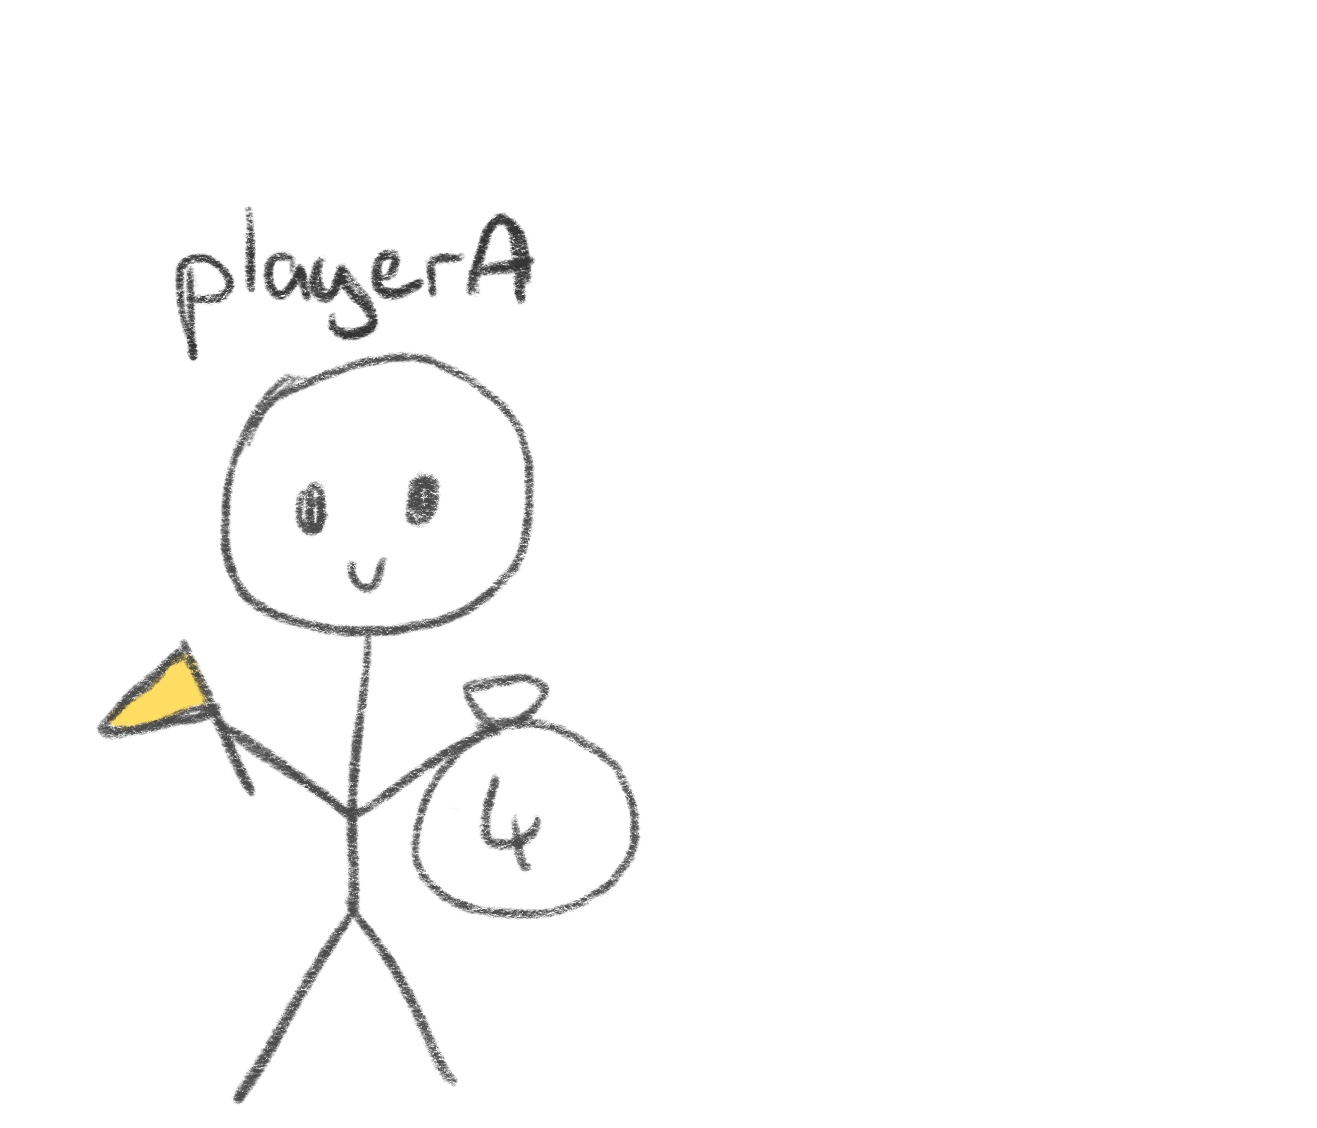
\includegraphics[scale=0.15]{img/0}
      \caption{Create}
    \end{figure}
  \end{frame}
  \begin{frame}{Approach: betting protocol}
    \begin{figure}
      \centering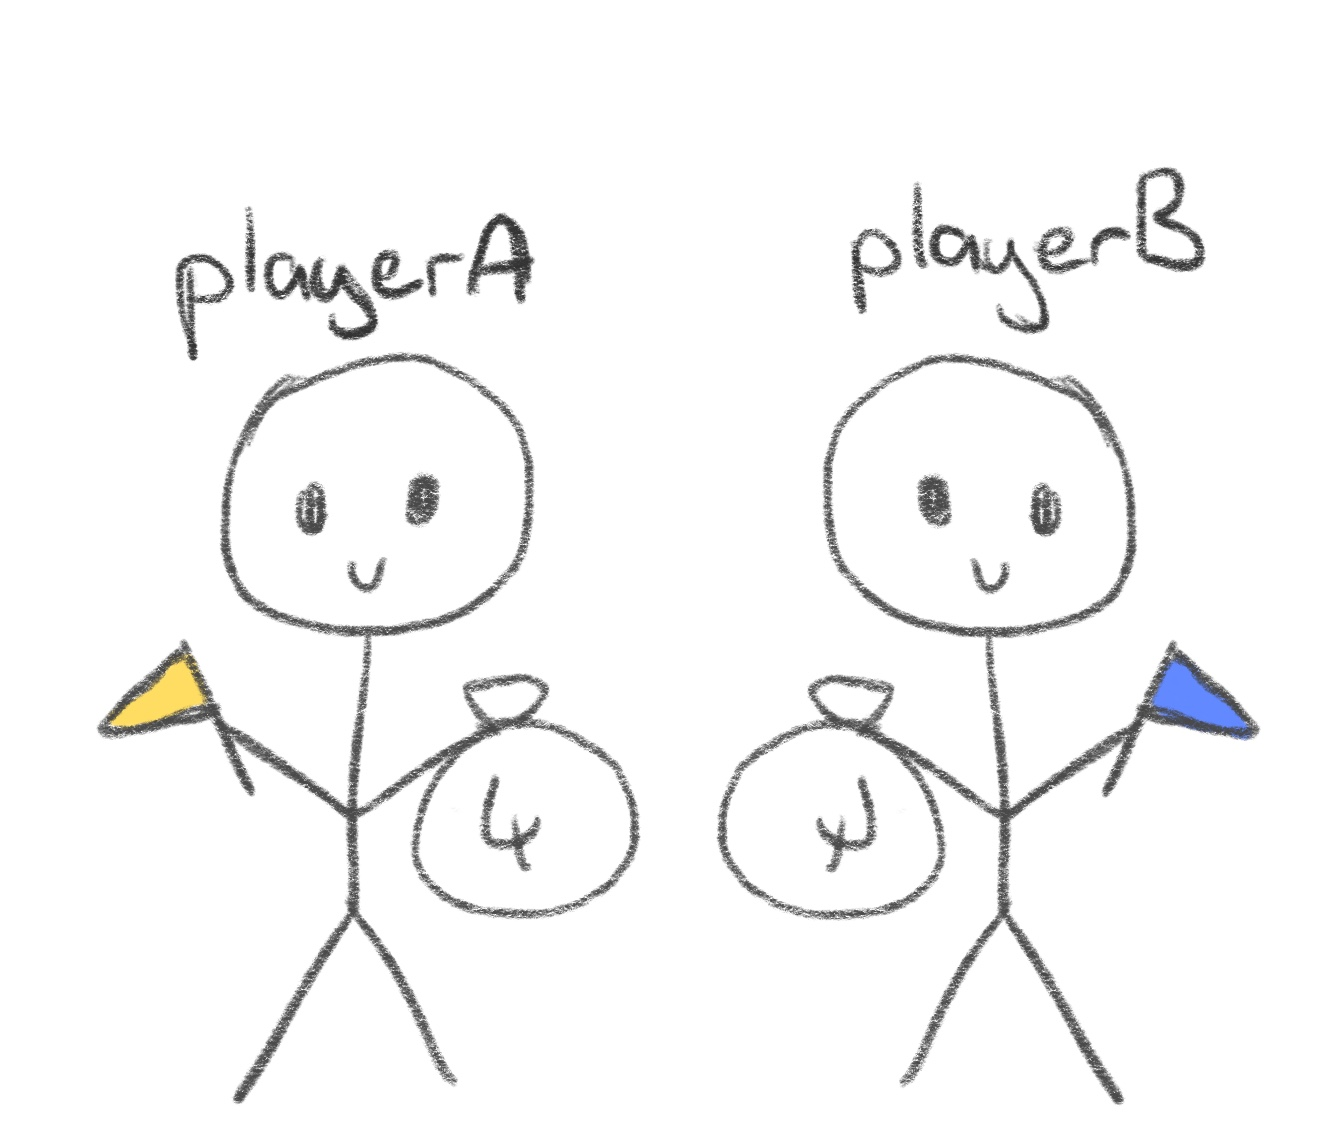
\includegraphics[scale=0.15]{img/1}
      \caption{Join}
    \end{figure}
  \end{frame}
  \begin{frame}{Approach: betting protocol}
    \begin{figure}
      \centering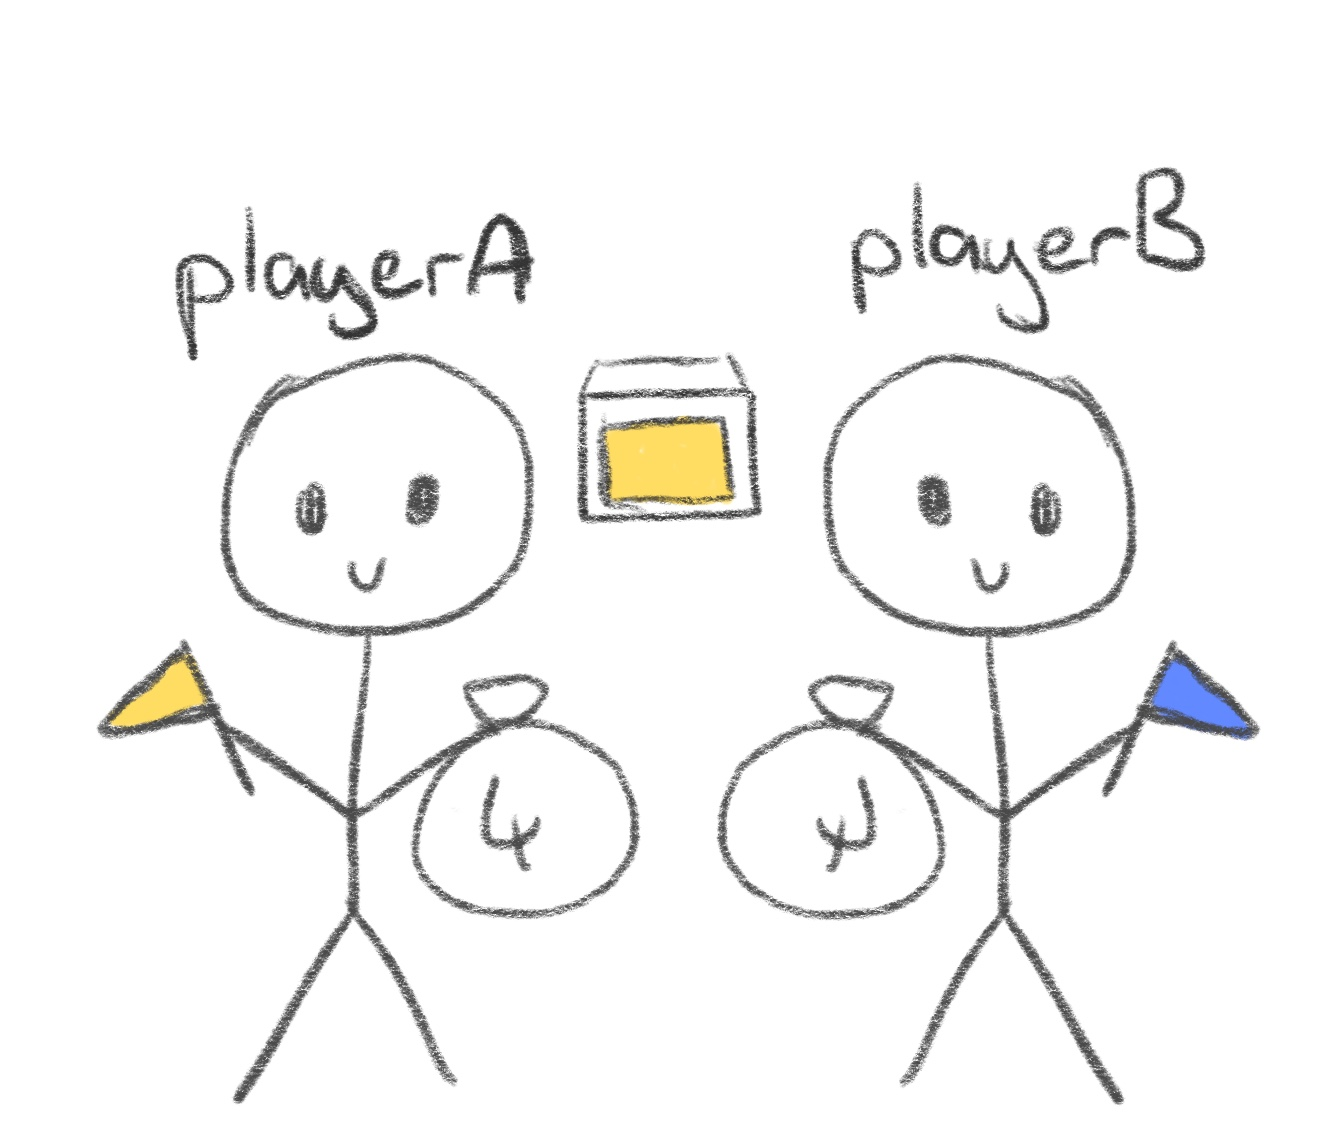
\includegraphics[scale=0.15]{img/2}
      \caption{Update}
    \end{figure}
  \end{frame}
  \begin{frame}{Approach: betting protocol}
    \begin{figure}
      \centering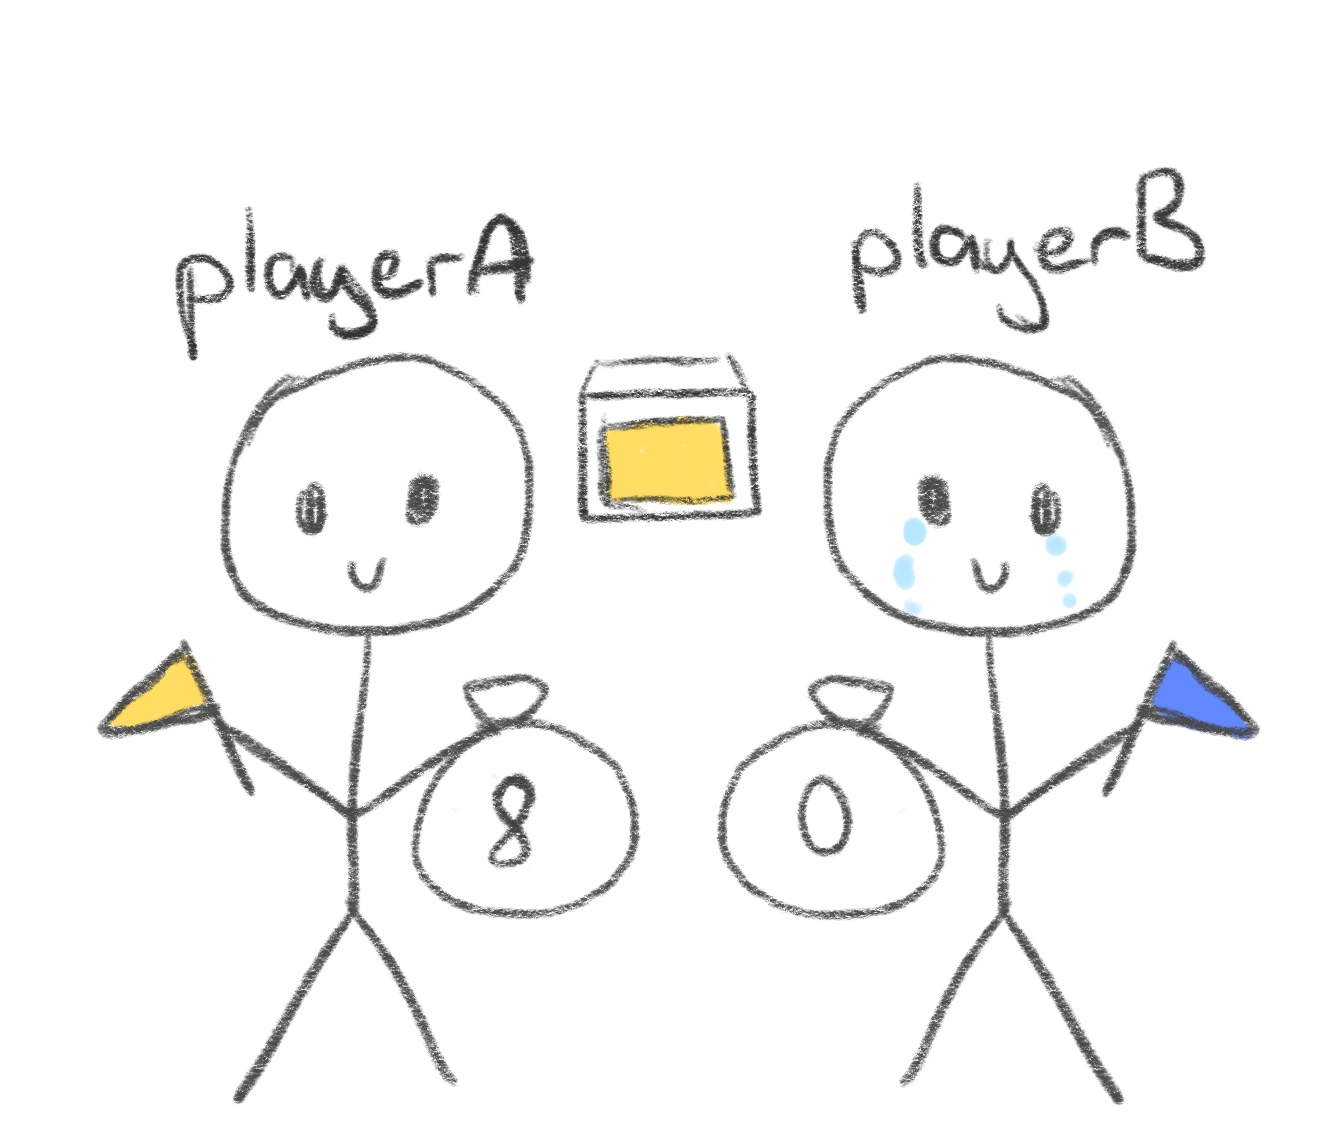
\includegraphics[scale=0.15]{img/3}
      \caption{Finalize}
    \end{figure}
  \end{frame}

  \begin{frame}{Approach: external data sources}
    How do we receive game results in a \emph{decentral} manner?\pause\\
    It's the Oracle problem!
  \end{frame}

  \begin{frame}{Approach: external data sources}
    \centering\alert{Chainlink} as the secure middleware between blockchain and real world
  \end{frame}

  \begin{frame}{Approach: external data sources}
    \begin{figure}[htbp]
      \centering
      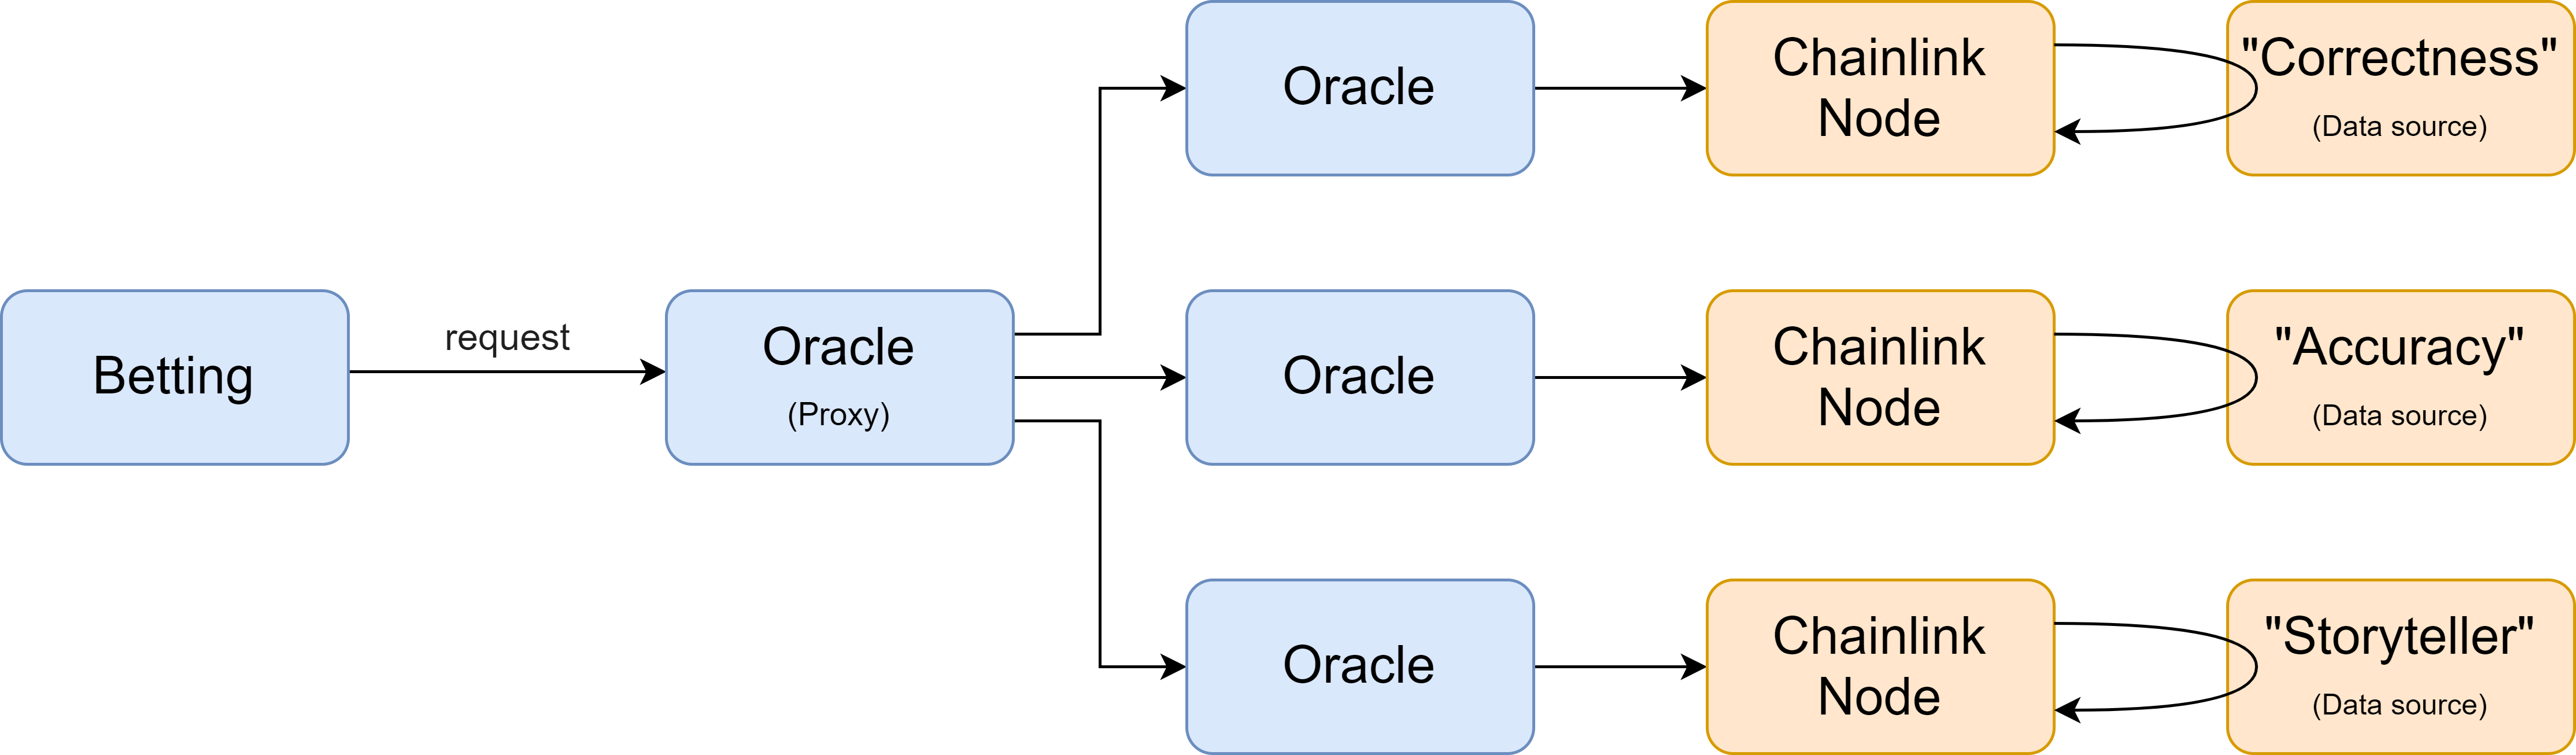
\includegraphics[scale=0.08]{img/oracle}
      \caption{Requesting data using a decentralized oracle network}
    \end{figure}
  \end{frame}

  \section{Demo}
  \begin{frame}{Approach: external data sources}
    \begin{figure}[htbp]
      \centering
      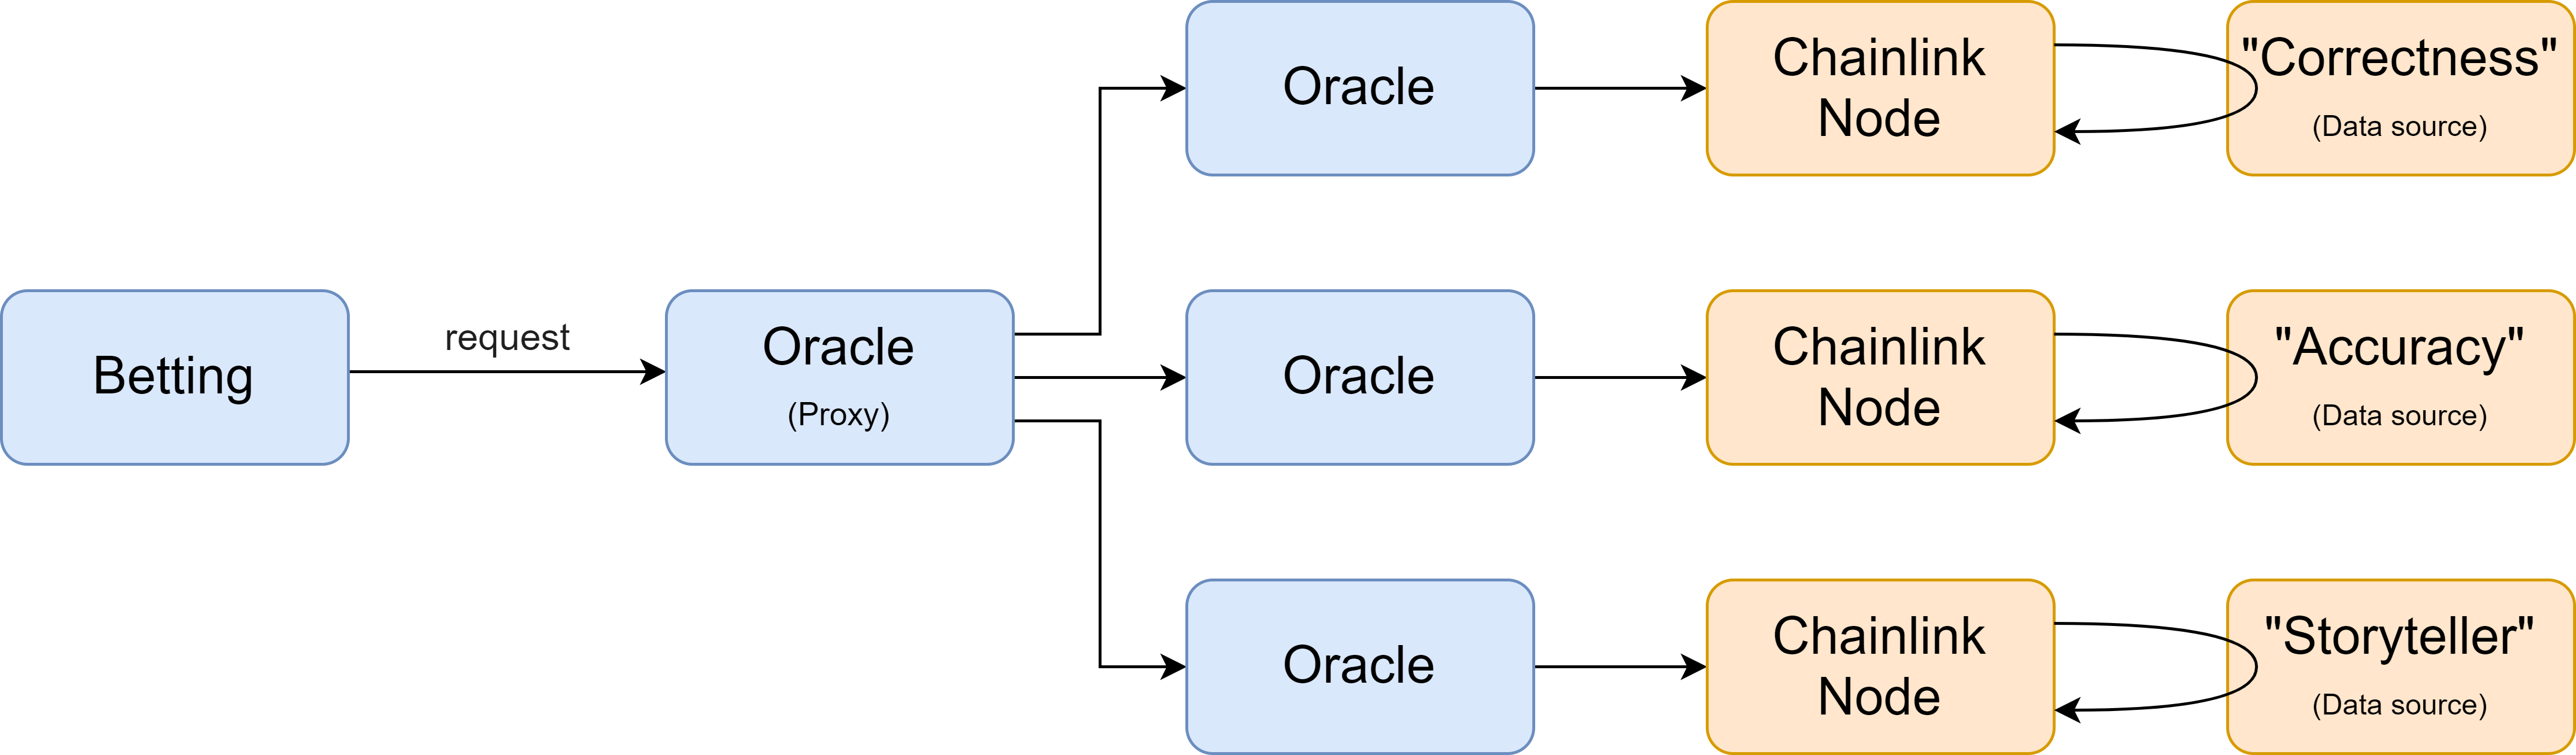
\includegraphics[scale=0.08]{img/oracle}
      \caption{Requesting data using a decentralized oracle network}
    \end{figure}
  \end{frame}

  \section{Hiccups and bugs}
  \begin{frame}{Hiccups and bugs}
    \begin{itemize}
      \item Development workflow fundamentally different
      \item Lots of things to consider and remember in order to have something working
      \item Web3 library sometimes seems almost like a separate programming language
      \item MetaMask seems to struggle with blockchain resets
    \end{itemize}
  \end{frame}
\end{document}
